\chapter{Background}
In this chapter, we will discuss about different forms 360 videos, then about the systems used for capturing each of these different forms. We then provide some necessary background to understand the image stitching pipeline.

\section{Different types of 360 Videos}
There are mainly ways 4 types of 360 capturing viz, monoscopic, Omni-directional Stereo(ODS), and Light Field cameras. In this work we will focus on monoscopic and stereoscopic cameras. 
\begin{figure}[h]
	\centering
	\begin{subfigure}{.5\textwidth}
		\centering
		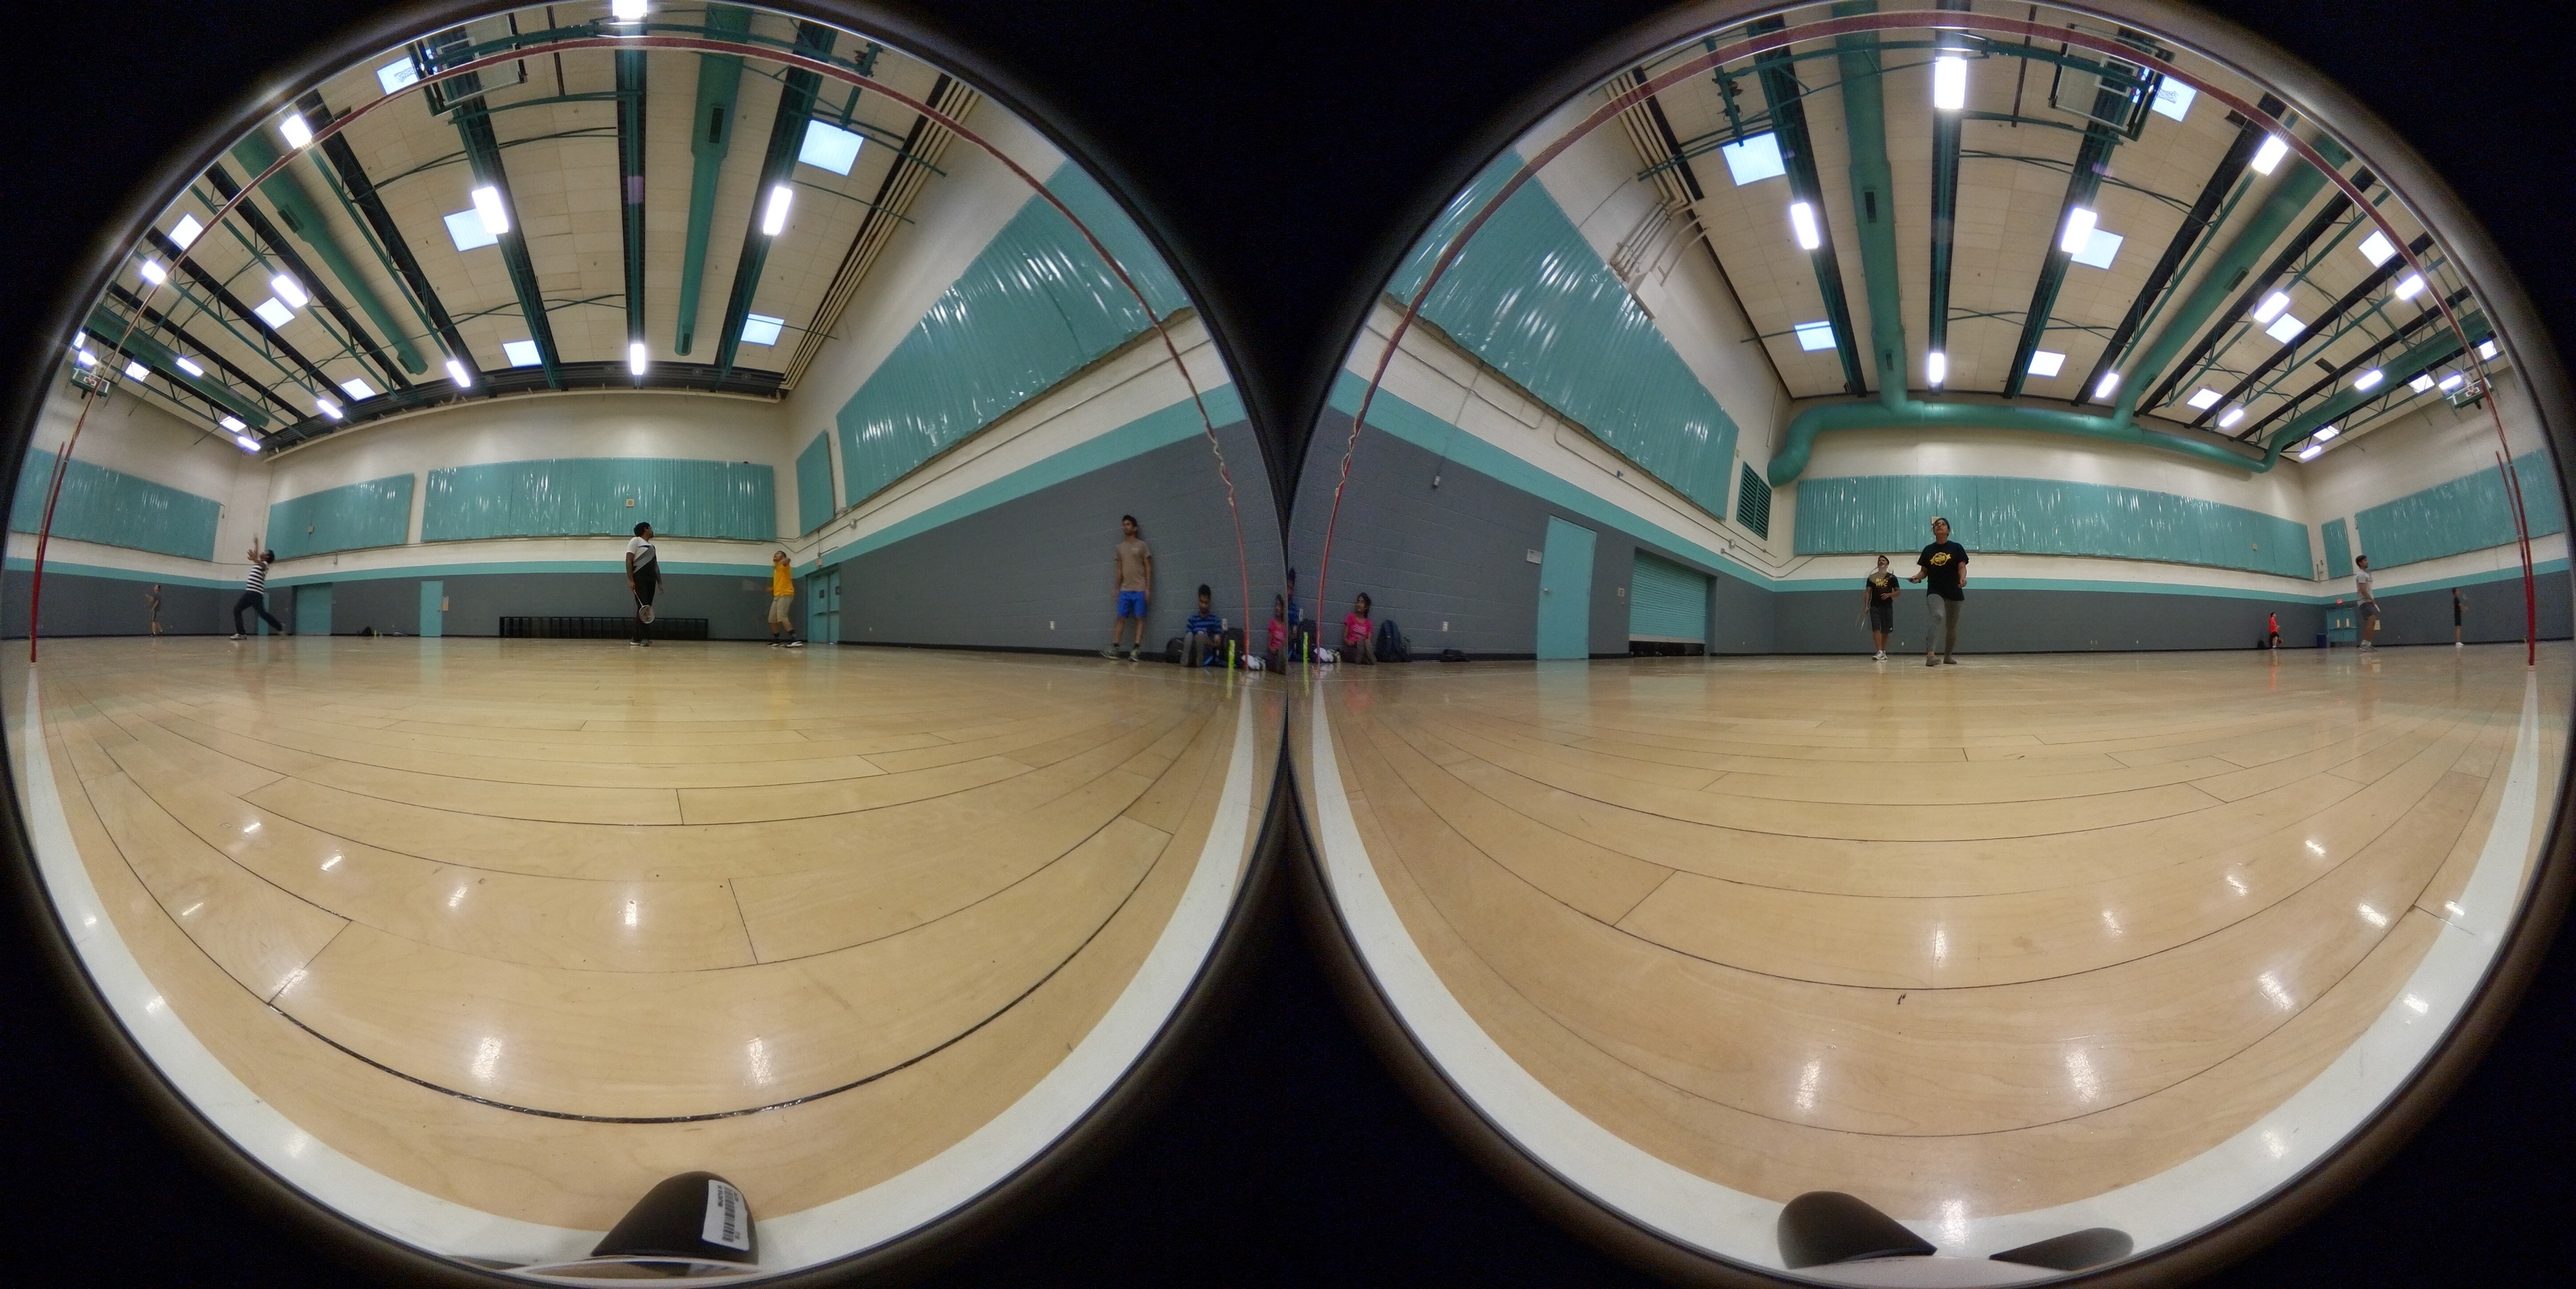
\includegraphics[width=1\linewidth]{/media/gunman/Data/thesis/ThesisLatex/data/images/fisheye_image_pair.jpg}
		\caption{Pair of spherical fisheye images}
		\label{fig:sub1}
	\end{subfigure}%
	\begin{subfigure}{.5\textwidth}
		\centering
		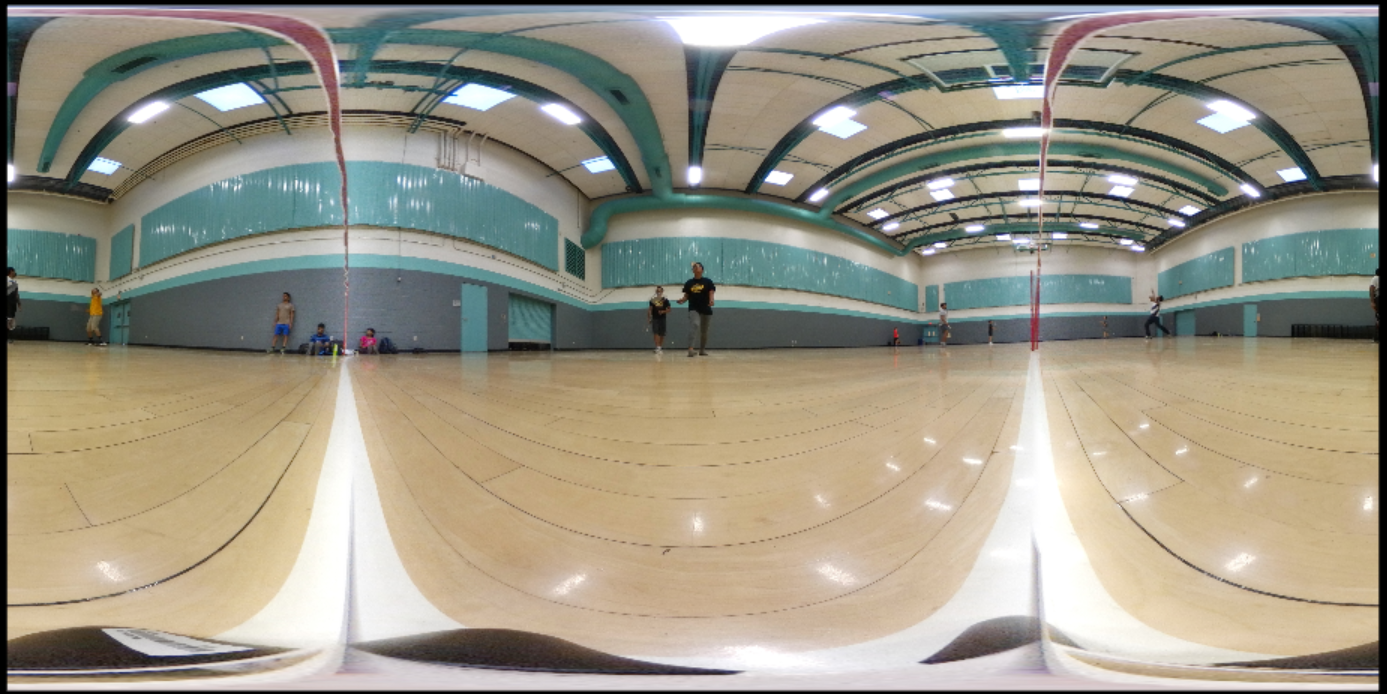
\includegraphics[width=1\linewidth]{/media/gunman/Data/thesis/ThesisLatex/data/images/fisheye_2_equirect.png}
		\caption{Equirectangular projected output}
		\label{fig:sub2}
	\end{subfigure}
	\caption{A 360 degree capture and corresponding panorama}
	\label{fig:test}
\end{figure}
\subsection{Monoscopic 360 Degree}
Fisheye lenses allow image sensors to capture images within an ultra-wide hemispheric field of view. With two fisheye-lensed sensors that capture complementary fields of view each of over 180\textdegree , the pair of captured images can be processed to achieve over a spherical 360\textdegree  x 180\textdegree  area, as shown in Figure x. The equirectangular projection format is a common format for 360\textdegree  x 180\textdegree  images, allowing remapping to other projections for convenient viewing. 



\subsection{Omni-directional Stereo(ODS)}
ODS output consist of two panoramas one for each eye, and provide the binocular stereo needed for perceiving depth information of the scene with respect to the view point of capturing device. In order to generate such output, we need to capture stereo information from all the viewing directions. Instead of capturing from all the viewing directions, we capture in certain directions, equally distributed over the 360 degree viewing angle and later process them to get the virtual camera viewpoints. We finally get the two panoramas one for each eye, which helps see the 360 view with depth.

\begin{figure}[h]
	\begin{center}
		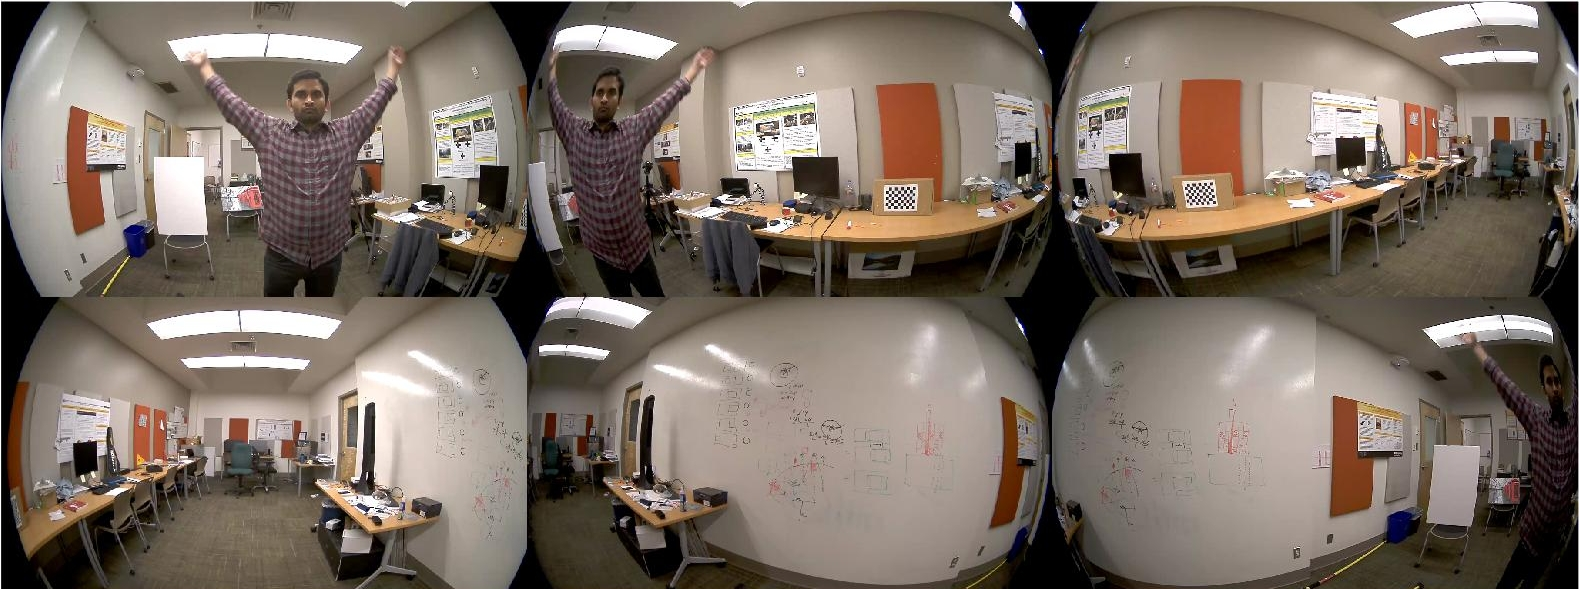
\includegraphics[width=1\textwidth]{/media/gunman/Data/thesis/ThesisLatex/data/images/fisheye_all6_cropped.jpg}
		\caption{Six camera views covering full 360 Hfov}
		\label{ODS_input}
	\end{center}
	\vspace{-0.3in}
\end{figure} 
\begin{figure}[h]
	\begin{center}
		\includegraphics[width=1\textwidth]{/media/gunman/Data/thesis/ThesisLatex/data/images/ODS_output.png}
		\caption{ODS panorama, one for each eyes.}
		\label{ODS_output}
	\end{center}
	\vspace{-0.3in}
\end{figure} 


%\section{Key Words}
%VR Panorama related:
%FOV:
%Binocular Stereo:
%Frame rate:
%Resolution:
%
%Camera Related:
%Pinhole Camera: 
%Fisheye:
%Equirectangular Projection:
%Camera Calibration Process:
%Intrinsics:
%Extrinsics:

%Stitching Algorithm Related:
%Optical Flow:
%Temporal Regularization:
%Pyramid:
%Video Compression: 
%
%Compression Related:
%Video Compression Terminology:
%Frame Types:
%JPEG Compression:
%Motion Blocks:
%Motion Vectors:

Image Representations:
RGB Vs HSV Vs YCbCr(YUV)
RGB is mainly for display's. HSV is easier as we have intensity channel is available. For vision applications intensity channel is very useful, for graphics people it's easier as they can change the Hue - color, Saturation - colorfulness(intensity of color, shades of color), value - overall intensity  intensity of image. Y'CbCr is used to mainly for storage and transmission efficiency. Y' - Luma, which is intensity of gamma corrected RGB image. We use gamma correction, which is non linear encoding of luminance/brightness to adjust for the way humans perceive light and color, i.e we perceive the variations in darkness more than the variations in brightness. And also we perceive light more than color.The more perceivable luma (Y') is used with high precision, whereas color(Cb Cr) can be of low precision, thereby reducing the size of the image.

%\section{Related Work:}
%
%%Status quo:
%%Existing 360 camera solutions. \newline
%%\cite{Milbeaut-ISP}
%Many have argued [Edvardo Hotmobile, Nvidia, AMD] that we need resolutions greater than 16k and frame-rate greater of 240 for true immersion in VR. At such higher framerate and resolutions there is lot of information that is redundantly captured, processed and transferred. Therefore, in our work, we study how the energy and latency of each stage get affected by the output resolution and the characterize the bottlenecks in greater detail. 
%
%%Existing systems \newline
%%Many existing systems like Google Jump, Facebook Surround capture and compute on enormous amount of data consuming several hundreds of watts of power to stitch images in realtime 30fps. 
%%Google Jump, Facebook Surround, Mega Stereo, Samsung Gear 360 \newline
%%Differentiating our work \newline
%%Bottlenecks in the existing systems \newline
%
%
%%Compression Related Work: 
%%Mobisys [Rubrix]
%%Conduit encoding:
%%https://avp.github.io/conduit/
%In this  project, they are using region based compression and other smart techniques. Although these works are for VR streaming, they share common techniques like reducing bandwidth by managing the image representation and decreasing latency by close integration of stages in VR streaming.
%%Pyramid encoding: https://code.facebook.com/posts/1126354007399553/next-generation-video-encoding-techniques-for-360-video-and-vr/
%%I think facebook's pyramid encoding seems a good idea for streaming, at that scale of facebook's needs. But I have some criticism for  cube projection, as they don't use region based compression. The pyramid encoding is a good technique though, to reduce image file size
%%
